\chapter{Background and Problem}

% - old ud-gf
% - newer naive approach - github + article 2017
%   - limitations
%   - performance


% Background to the assignment. Why is it relevant?
\section{Background}
%   -> useful synthesis: UD-GF
%   -> applications:
%     - translation  - CL 2020
%     - semantics    - CL 2020
%     - concept alignment - Arianna
%     - SMU work - analysis of real-world law text

There exists a proof-of-concept implementation of a tool for converting between the trees for GF and UD,
with the help of so-called labels-files which describe the mapping between UD labels and GF functions,
called gf-ud, which contains both a component for converting from UD to GF, called ud2gf\cite{kolachina-ranta-2017}\footnotemark[1]
and a component for converting from GF to UD, called gf2ud\cite{kolachina-ranta-2016}\footnotemark[1]. This work will focus on the ud2gf component.

\footnotetext[1]{These references apply to an older version of gf-ud, from before the one this thesis is based on. A part of the goal of this thesis is to document the later version in addition to documenting the changes made in the process of this thesis.}

% \todo{these references apply to an older version of gf-ud, from before the one I was working on. a part of the goal of this thesis is to document the old-new version that my changes was based on}

% The labels files can also contain macros, which allows constructing virtual GF functions during the translation from UD, which will be expanded to real GF functions at the end of the translation.
% These can, among other uses, be used to preserve information from the UD labels about subtrees, which can then be used at later points of the transformation to ensure that the desired GF tree is produced.

The gf-ud tool has been used for both translation and semantics\cite{ranta2020abstract}. %\todo{actually explain this}
Another application has been in concept alignment\cite{masciolini2021grammar}.
There has also been work using it for analysis of law text for the purpose of making a Controlled Natural Language for law\cite{listenmaa-etal-2021-towards}.

\section{Problem}
% The formulation of the problem at hand and, the assignment. This should include an extended version of the scientific problem definition and references to knowledge within the area given in the thesis proposal.

% What has been done before and what remains to be done

% 2. Background & Problem
% - old ud-gf
% - newer naive approach - github + article 2017
%   - limitations
%   - performance

The current ud2gf implementation has some limitations. There are three main problems this work tries to fix.

The first problem is that it quickly becomes extremely slow for sentences with more than a couple of words and/or
when using large GF-grammars, e.g. GF-grammars containing Wordnet\cite{angelov2016predicting}. \\
The second problem is that if the structure differs too much between the representation of a sentence in UD format and as a GF tree, it is not possible to describe the required transformation in the current "labels file" language. See section \ref{sect:flex} below for more details. \\
The third problem is that it can sometimes be difficult to figure out why a rule in a labels-file is not firing, so it would be useful to have a debugging tool to help diagnosing such issues.


\subsection{Flexibility}\label{sect:flex}

As an example of a phrase that can be difficult to convert using the old gf2ud, let us consider the adjectival phrase "cute, fluffy and furry"
would be described in UD format as in Figures \ref{fig:ud_cute_text} and \ref{fig:ud_cute}.


\begin{figure}
    \begin{verbatim}
    1  cute  cute  ADJ  JJ  Degree=Pos  0  root  _  FUN=cute_A
    2  ,  ,  PUNCT  ,  _  3  punct  _  _
    3  fluffy  fluffy  ADJ  JJ  Degree=Pos  1  conj  _  FUN=fluffy_A
    4  and  and  CCONJ  CC  _  5  cc  _  FUN=and_Conj
    5  furry  furry  ADJ  JJ  Degree=Pos  1  conj  _  FUN=furry_A
    \end{verbatim}
    % \begin{tabular}{|c|c|c|c|c|c|c|c|c|c|}
    % \hline
    % 1 & cute & cute & ADJ & JJ & Degree\=Pos & 0 & root & \_ & FUN\=cute\_A \
    % \hline
    % 2 & , & , & PUNCT & , & \_ & 3 & punct & \_ & \_ \
    % \hline
    % 3 & fluffy & fluffy & ADJ & JJ & Degree\=Pos & 1 & conj & _ & FUN\=fluffy\_A \
    % \hline
    % 4 & and & and & CCONJ & CC & \_ & 5 & cc & \_ & FUN\=and\_Conj \
    % \hline
    % 5 & furry & furry & ADJ & JJ & Degree\=Pos & 1 & conj & \_ & FUN\=furry\_A \
    % \hline
    % \end{tabular}
    \caption{The phrase "cute, fluffy and furry" as a textual UD tree}
    \label{fig:ud_cute_text}
\end{figure}

\begin{figure}
    \centering
    % \begin{dependency}
  \begin{deptext}[column sep=0.4cm]
      cute \& , \& fluffy \& and \& furry \\
    {\tt ADJ}\&{\tt PUNCT}\&{\tt ADJ}\&{\tt CCONJ}\&{\tt ADJ} \\
  \end{deptext}
  \depedge{2}{1}{punct}
  \depedge{0}{2}{conj}
  \depedge{4}{3}{cc}
  \depedge{0}{4}{conj}
\end{dependency} \\
    % \includesvg{ud-annotatrix-corpus.svg}
    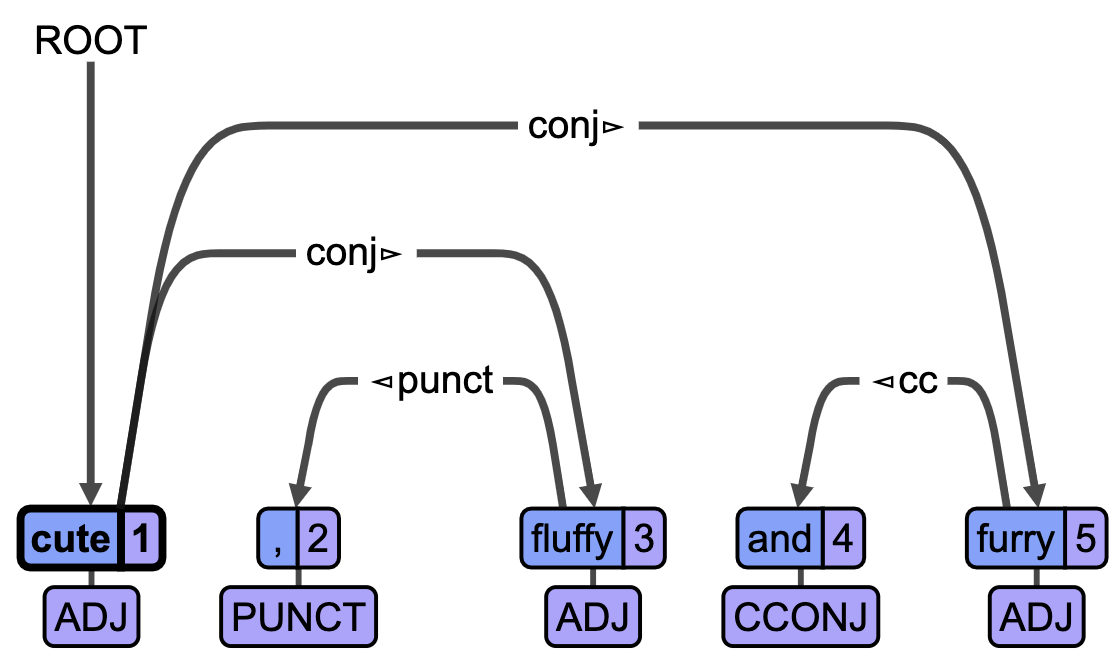
\includegraphics[width=0.7\textwidth]{ud_cute.png}
    \caption{The phrase "cute, fluffy and furry" as a UD tree in graphical format}
    \label{fig:ud_cute}
\end{figure}
% \include{}

\begin{figure}
    \centering
    % \begin{dependency}
  \begin{deptext}[column sep=0.4cm]
      cute \& , \& fluffy \& and \& furry \\
    {\tt ADJ}\&{\tt PUNCT}\&{\tt ADJ}\&{\tt CCONJ}\&{\tt ADJ} \\
  \end{deptext}
  \depedge{2}{1}{punct}
  \depedge{0}{2}{conj}
  \depedge{4}{3}{cc}
  \depedge{0}{4}{conj}
\end{dependency} \\
    % \includesvg{ud-annotatrix-corpus.svg}
    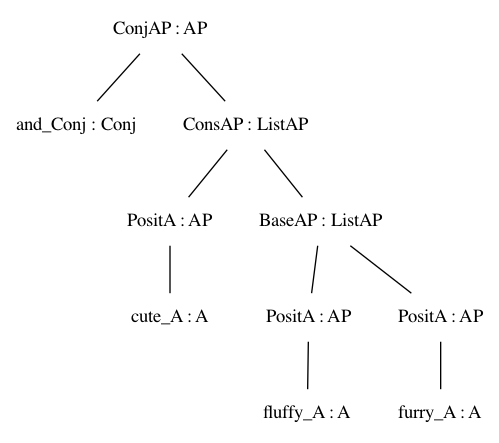
\includegraphics[width=0.7\textwidth]{cute_gf.png}
    \caption{The phrase "cute, fluffy and furry" as a GF tree in graphical format. }
    \label{fig:gf_cute}
\end{figure}

The GF version of the same tree, shown in Figure \ref{fig:gf_cute}, would look like this:

\begin{verbatim}
ConjAP and_Conj (ConsAP (PositA cute_A)
                        (BaseAP (PositA fluffy_A) (PositA furry_A)))
\end{verbatim}
Here we can see that in UD, the word "cute" is in the root, while the conjunction "and" is at the bottom of the tree, while in GF the conjunction is a direct child of the root. This transformation can not be preformed by the simple single-layer transformations that are available in the current macro-system for labels files.

% Ideas:
%
% - Limits on how to transform trees - solution: extend language. currently hack using lambda calculus, but maybe better macros
%
% - Evaluate effectiveness of tool
%
% - (somewhere mention the performance boosts and analyse the complexity of it)

% This section is optional. It may be used if there is a need to describe the problem that you want to solve in more technical
% detail and if this problem description is too extensive to fit in the introduction.

% From elsewhere:
% - Background: GF \cite{ranta-2004}, UD \cite{nivre-etal-2016-universal},
%   - previous work: gf2ud \cite{kolachina-ranta-2016}, ud2gf \cite{kolachina-ranta-2017}
% - Describe the new algorithm
% - Extending the macro language
%   - Need for improvement: to match "fluffy and cute" needs 2 levels of nesting
%   - Solution: continuations
% - Case study: legal language

The translation described by a labels file is not one-to-one and there are often many possible GF trees that a UD tree could be translated to. The possible trees are currently ranked by completeness, as in how many of the words are included in the generated tree. However this ranking is incomplete and in case two possible trees, with the same GF category, cover the same words, an arbitrary tree will be chosen. A better choice could be to also check the linearization of these trees and rank those whose linearization is more similar to the original string higher. It would also be possible to completely exclude trees with differing linearization, but that would run counter to the goal of robustness.


% 3. The new algorithm
% - definitions
% - examples
% - how annotations work

% \section{Context}
% \todo[inline]{What's the difference between this and intro?}
% This work is mostly a continuation of the work in \cite{kolachina-ranta-2017}.

% A practical problem for which this tool can be useful can be found in \cite{listenmaa-etal-2021-towards}. In the Future Work section, under "Robust fall-back options", gf2ud is mentioned as a possible solution to making the parser more robust.

% % Use one or two relevant and high quality references for providing evidence from the literature that the proposed study indeed
% % includes scientific and engineering challenges, or is related to existing ones. Convince the reader that the problem addressed
% % in this thesis has not been solved prior to this project.
